\chapter{Progettazione}
\label{cap:progettazione}

\section{Scopo del capitolo}
Successivamente all'apprendimento del background tecnologico, sono state improntate le basi dell'architettura del progetto, definendo lo schema del database su cui si poggia l'API e i concetti base del progetto.\\
Nei seguenti paragrafi verrà quindi trattata l'architettura e le configurazioni utilizzate che funzionano da base per l'implementazione di quanto sviluppato.\\

\section{Architettura REST}
L’architettura REST, acronimo di “Representational State Transfer”, è un approccio di progettazione per la creazione di servizi web che si basa sui principi dell’HTTP (Hypertext Transfer Protocol).\\
Le principali caratteristiche di un’architettura REST includono:
\begin{itemize}
\item \textbf{Sistema client-server}, dove il client è chi fa le richieste e il server fornisce le risposte;
\item \textbf{Sistema layered},perchè possono essere composte da più livelli di servizi indipendenti;
\item \textbf{Stateless}, significa che il server non contiene client state, quindi ogni richiesta ha abbastanza informazione per il server per processarla;
\item \textbf{Cacheable}, significa che l’architettura può memorizzare le risposte dei server e riutilizzarle;
\item \textbf{Resource-based}: questo approccio è considerato tale, dato che si concentra sull’identificazione e la gestione delle risorse all’interno di un sistema. Le risorse vengono identificate da degli URI ed esse possono essere create,aggiornate,richieste o eliminate (operazioni CRUD) attraverso operazioni HTTP standard (POST,PUT,GET,DELETE);
\item \textbf{Manipolazione delle risorse}, poichè le risorse sono diverse dalla loro rappresentazione logica, utilizzando formati come JSON o XML.
\end{itemize}
Questo stile architetturale è utilizzato soprattutto per la realizzazione di API poichè l'adozione dei principi standard di HTTP mantiene un'interfaccia uniforme e l'approccio resource-based ne semplifica la progettazione, dato che le risorse vengono identificate da URI\textsubscript{g}.

\subsection{Convenzioni di denominazione REST}
Buona prassi nella creazione di un'API REST è il rispetto di convenzioni per la nomenclatura degli endpoint\textsubscript{g}. Sebbene non esista un'unica convenzione obbligatoria, esistono delle best practices per garantire una facile lettura e comprensibilità per agevolare gli sviluppatori che adoperano l'API.\\
Le seguenti convenzioni sono state rispettate nella progettazione dell'API:
\begin{itemize}
\item  pluralizzare le risorse, per distinguere se si fa riferimento ad una lista di una determinata risorsa o ad una singola risorsa;
\item usare lettere minuscole;
\item non usare estensioni dei file;
\item in caso di nomi composti utilizzare il "-";
\item non usare underscore;
\item non utilizzare abbreviazioni o slang;
\item non utilizzare verbi, poichè l'azione dovrebbe essere indicata dal metodo HTTP utilizzato.
\end{itemize}

\section{Spring MVC}
Nello sviluppo di una API REST tramite Spring Boot è comune l'utilizzo del pattern architetturale Model-View-Controller(MVC).\\

\begin{figure}[H] 
    \centering 
    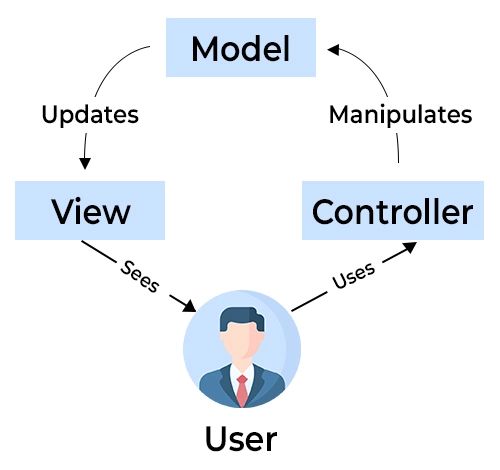
\includegraphics[width=0.50\columnwidth]{mvc2} 
    \caption{Schema Model-View-Controller}
\end{figure}

\subsection{Model}
Il Modello o Model in inglese,appresenta i dati e i metodi per accedere ai dati dell'applicazione. Se esso viene aggiornato in seguito ad azioni o eventi, notificherà la View e il Controller del cambiamento.\\
Nel contesto dello sviluppo di un'API REST, il Model contiene dati che vengono elaborati e restituiti dall'API.\\
All'interno del progetto il Model è formato dai seguenti elementi.
\subsubsection*{Entità}
Le entità sono risorse rappresentate con classi Java segnate con l'annotazione\textsubscript{g} \textit{@Entity}. Utilizzando questa annotazione si identifica che quella classe è mappata\textsubscript{g} ad una tabella del database. Esse dichiarano al loro interno, tramite annotazioni JPA apposite, gli attributi corrispondenti alla tabella a cui fa riferimento e, altre annotazioni per mantenere le relazioni presenti nel database tra le tabelle.
\subsubsection*{Repository}
Le repository implementate nel progetto gestiscono l'accesso ai dati e definiscono metodi per eseguire operazioni di base sui dati, come l'inserimento, la modifica, la cancellazione e la ricerca. Tutto questo estendendo interfacce JPA, che consentono di eseguire operazioni in una base di dati senza scrivere codice SQL o query.
\subsubsection*{DTO}
Data Transfer Object (DTO), oggetti utilizzati per modellare le rappresentazioni dei dati, utilizzati per definire sia i dati inviati dal client nelle requests che quelli che inviati dal server al cliente nelle responses.\\

\subsection{View}
La Vista o View in inglese, è responsabile di mostrare i dati provenienti dal Model e dell'interazione con l'utente. Essa cattura gli input dell'utente e delega al Controller l'elaborazione.\\
Dato che il progetto si concentrava sul lato back-end, precisamente sullo sviluppo dell'API REST, non ho quindi sviluppato una vera e propria View, poichè l'output è in formato JSON. In questo contesto l'output prodotto contenente i dati presentati al client in formato JSON, potrebbe essere considerata come "View".\\

\subsection{Controller}
Il Controller gestisce il flusso dell'applicazione. Esso riceve i comandi dell'utente attraverso la View e reagisce eseguendo operazioni conseguenti. Queste sue operazioni possono o meno coinvolgere il Model, ma portano generalmente sempre ad un cambiamento di stato della View.\\
All'interno del meccanismo di Spring MVC il Controller gestisce le richieste HTTP in arrivo, selezionando il Controller adeguato e assegnato a quell'endpoint API. Sono quindi responsabili di ricevere le richieste, elaborarle e restituire le risposte corrispondenti.\\
Per identificare il metodo associato ad una determinata operazione HTTP, vengono utilizzate le seguenti annotazioni \textit{@PostMapping}, \textit{@GetMapping}, \textit{@PutMapping}, \textit{@PatchMapping} e \textit{@DeleteMapping}. 
All'interno del progetto il Controller è formato dai seguenti elementi.
\subsubsection*{Controller}
I Controller contengono i metodi a cui vengono associati i percorsi delle richieste HTTP. Esso interpreta i parametri che possono provenire dall'URL o dal corpo della richiesta(parametri di query o dati JSON). Internamente a questi metodi viene richiamato il Service appropriato per eseguire operazioni di business logic al risultato finale da restituire.\\
Per garantire che i dati inseriti dagli utenti o provenienti da richieste siano conformi alle aspettative e non causino errori vengono inseriti dei controlli di validazioni all'interno dei metodi del Controller.
\subsubsection*{Service}
I Service eseguono operazioni complesse ed elaborazioni di dati, gestendo la business logic dell'applicazione. Essi interagiscono con i Repository per recuperare dati dal database e vengono richiamati all'interno dei metodi del Controller.
\subsubsection*{Exception Handler}
Per centralizzare la gestione delle eccezioni è stato creato un handler che garantisce uniformità alle eccezioni che l'applicazione può produrre.\\


\section{Pattern Client-Server}
\begin{figure}[H] 
    \centering 
    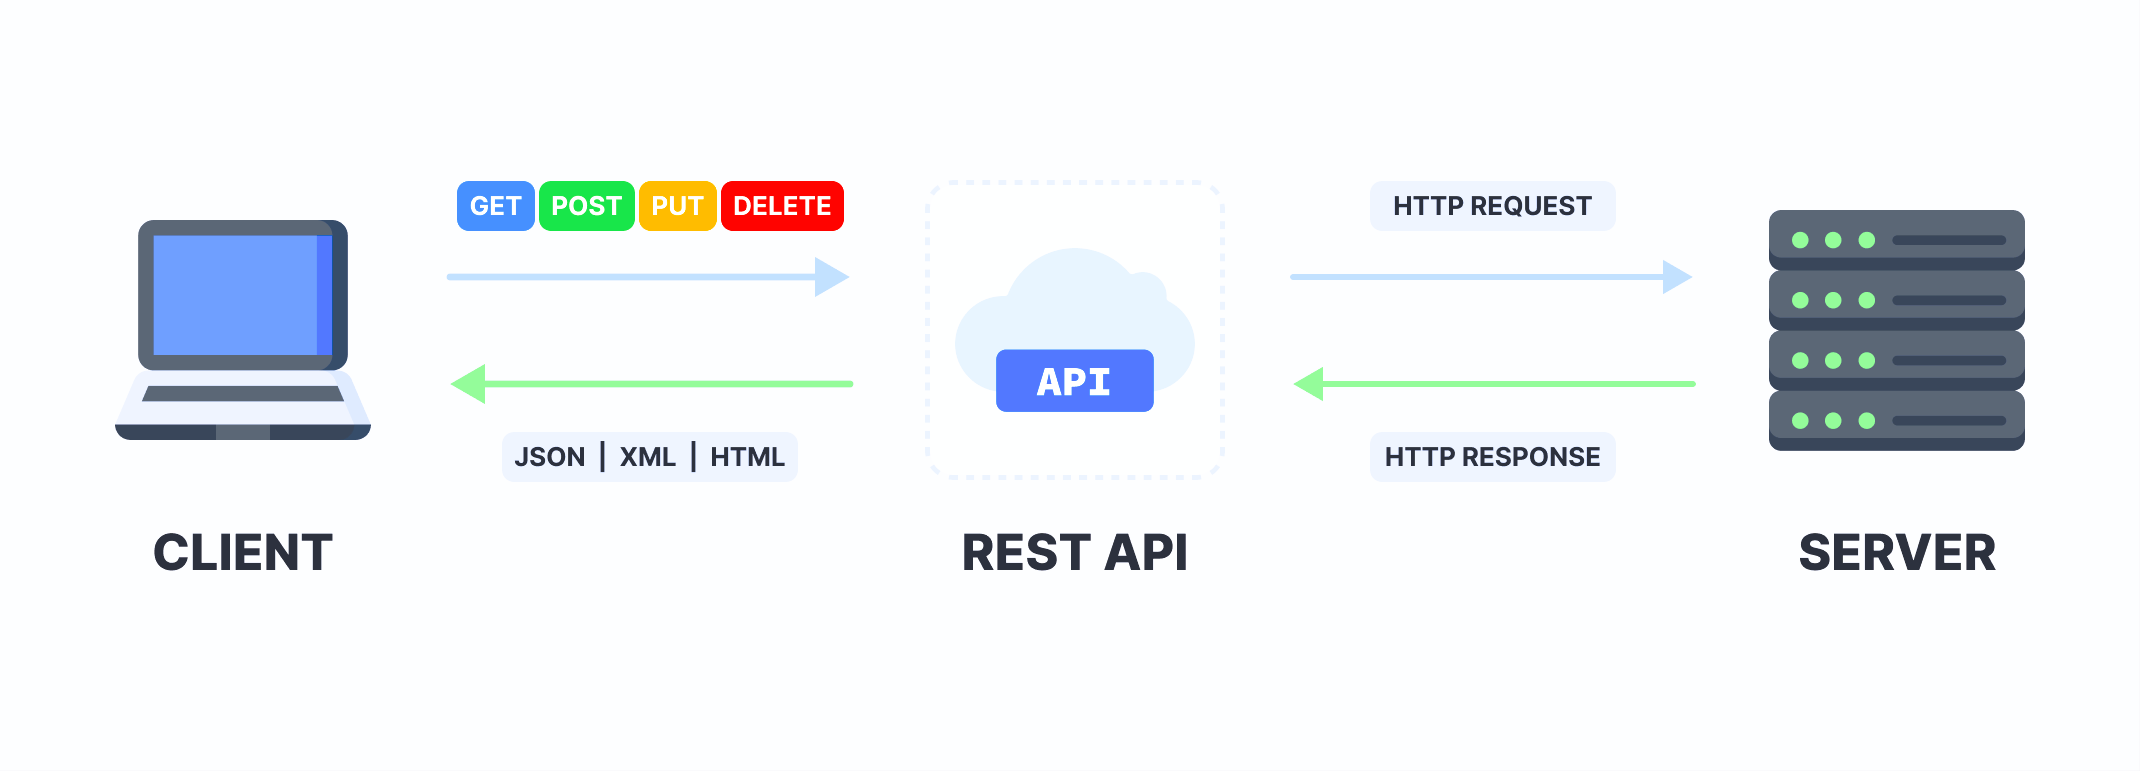
\includegraphics[width=0.90\columnwidth]{client-server} 
    \caption{Client-Server in una REST API}
\end{figure}
È un pattern architetturale composto da due componenti: client e server. Il client rappresenta il richiedente del servizio, mentre il server fornisce i contenuti e i servizi ai client, restando in attesa delle loro richieste.\\
Il pattern client-server si adatta perfettamente ad una API REST e le sue componenti sono identificate in questo modo.
\subsection*{Client}
In questo contesto il client è rappresentato da applicazioni o servizi che comunicano con l'API REST, inviando le richieste HTTP al server per ottenere quanto richiesto. Il client invia richieste utilizzando verbi standard HTTP per accedere alle risorse e alle funzionalità che l'API offre.
\subsection*{Server} 
Il server invece è colui che gestisce le richieste HTTP ricevute e genera le risposte in formato JSON. Esso quindi elabora le richieste ed interagisce col database per recuperare le informazioni.\\

\section{Design Pattern}
\label{cap:design pattern}
Nel prodotto sviluppato possiamo notare i seguenti Design Pattern.
Ad eccezione dell'ultimo Design Pattern adottato, in riferimento all'elenco sottostante, i restanti Design Pattern sono già implementati da Spring e Spring Boot.
\subsection*{Repository pattern}
Repository è un pattern ideato per dividere le operazioni di business logic da quelle di persistenza dei dati. Questo pattern fornisce astrazione ai dati nascondendo i dettagli di accesso, facilita il testing, supporta diverse sorgenti di dati e mantiene un codice riutilizzabile in quanto non sarà necessario modificare ampiamente il codice in caso di modifiche alla sorgente dati.\\
In Spring Boot vengono implementate interfacce annotandole con  l'annotazione \textit{@Repository} ed estendendole con interfacce JPA che permettono l'utilizzo di metodi che forniscono query basilari o la possibilità di creare metodi custom per query personalizzate.
\subsection*{Dependency Injection}
Dependency Injection è un pattern che inietta una dipendenza in una classe senza sapere l'implementazione effettiva. Questo può avvenire attraverso constructor injection, setter injection o method injection. Gli obiettivi di questo pattern sono: eliminare il forte accoppiamento tra le classi, rendere il codice più manutenibile e più facile da testare.\\
In Spring Boot risulta evidente tramite l'utilizzo di annotazioni come \textit{@Autowired}, iniettando direttamente le dipendenze necessarie, promuovendo il concetto successivo di Inversion of Control;
\subsection*{Inversion of Control}
Inversion of Control (IoC) è un design pattern nato sul concetto di invertire il controllo del flusso del sistema nella gestione delle dipendenze e del controllo interno di un'applicazione. Normalmente è l'applicazione che controlla le dipendenze o il flusso di esecuzione, ma questa responsabilità, utilizzando questo pattern, viene trasferita ad un framework. Il framework instanzierà oggetti, inietterà le dipendenze e coordinerà il flusso di esecuzione.\\
Spring Boot è costruito proprio su questo concetto chiave. Esso è correlato a IoC per i seguenti motivi:
\begin{itemize}
\item Component scan, esegue automaticamente uno scan delle classi individuando quelle contrassegnate con annotazioni come \textit{@Service}, \textit{@Repository}, \textit{@Controller} e altre;
\item Semplifica la gestione delle dipendenze, fornendo degli insiemi di dipendenze utili per determinate tecnologie sotto il nome di "starters", velocizzando l'inizializzazione delle dipendenze senza doverle configurare manualmente, fornendo un senso di controllo sulla configurazione iniziale;
\item Dependency Injection;
\item Application Context, agisce come contenitore per i bean\textsubscript{g} dell'applicazione. Esso gestisce i loro cicli di vita e inietta le dipendenze nei punti appropriati.
\end{itemize}
\subsection*{Front Controller}
Il Front Controller è un design pattern che permette di centralizzare la gestione delle richieste all'interno di un'applicazione. In Spring MVC è implementato dal framework per gestire le richieste HTTP verso il Controller adeguato.
\subsection*{Data Transfer Object}
Data Transfer Object (DTO) è un pattern utilizzato per gestire il trasferimento dei dati tra client e server. Gli obiettivi principali del pattern sono:
\begin{itemize}
\item Sicurezza, in quanto puoi controllare cosa si invia;
\item Flessibilità, puoi adattare i DTO in base alle esigenze dell'API;
\item Separano la rappresentazione interna da quella esterna dei dati.
\end{itemize}
Nel contesto di una API REST, i DTO vengono utilizzati sia nella Request che nella Response. Vengono utilizzati in entrambi i punti perchè quando il client invia dei dati magari non necessita degli oggetti completi ma solo di alcune informazioni. Invece quando il server restituisce dei dati il client se li può aspettare sotto una determinata struttura.\\




\section{Progettazione del database}
\subsection{Configurazione di Docker}
I container Docker offrono un'isolamento completo dell'ambiente, che aiuta a evitare conflitti di dipendenze e interferenze con altre applicazioni o servizi che potrebbero essere presenti sul sistema. Per questo motivo si è deciso di utilizzare l'approccio di sandboxing\textsubscript{g} che offre Docker, poichè l'utilizzo di container consente di isolare le applicazioni e i servizi in ambienti virtualizzati, condividendo il kernel del sistema operativo host ma separando le loro risorse e i loro processi.\\
Dato che le tabelle di mia creazione dovevano integrarsi con il database aziendale, tramite il tool Docker Compose\textsubscript{g} e un file di configurazione \textit{docker-compose.yaml}, è stato possibile avviare un nuovo container contenente un'immagine di Microsoft SQL Server, che forniva un backup del database aziendale con dati e tabelle.\\

\subsection{Modello dati}
\textbf{IMMAGINE UML SENZA ATTRIBUTI}\\

\noindent Nel seguente disegno si può notare il database su cui poggia l'API.\\
È stata inserita una nomenclatura <<esterna>> per indicare le tabelle proveniente dal database aziendale.\\
Di seguito elenco le tabelle da me create, spiegandone l'utilizzo e gli attributi:\\

\noindent \textbf{TUTTE LE TABELLE MIE}\\



\section{Configurazione iniziale del progetto}
\subsection{Spring Initializr}

\begin{figure}[!h] 
    \centering 
    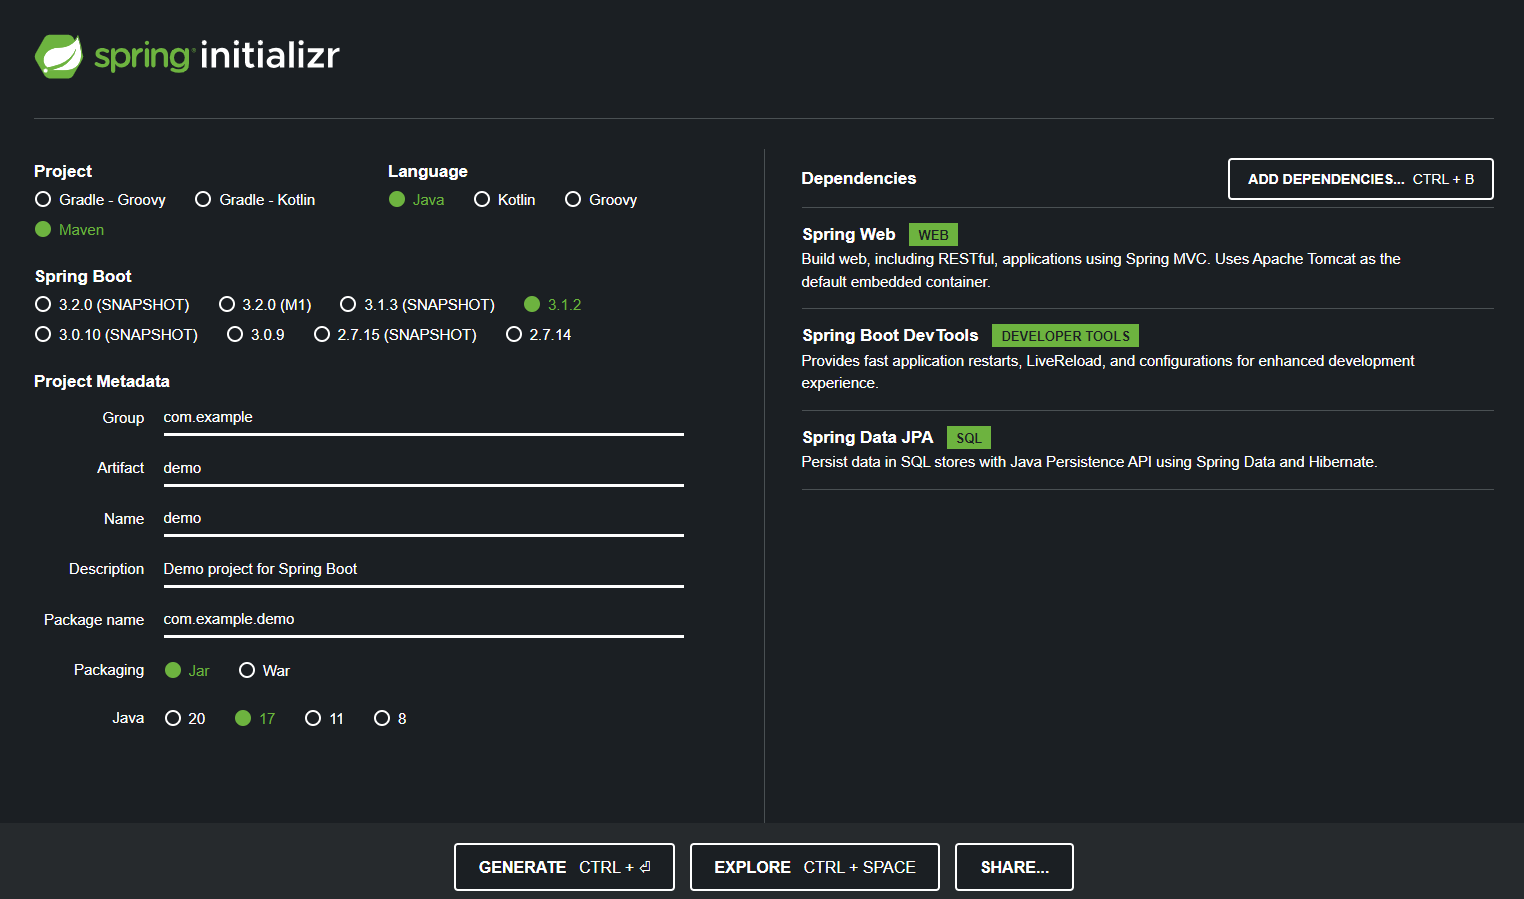
\includegraphics[width=0.95\columnwidth]{Spring_initializr} 
    \caption{Interfaccia Spring Initializr}
\end{figure}

\noindent \href{https://start.spring.io/}{Spring Initializr} è uno strumento online fornito dalla community di Spring Framework, che consente di creare rapidamente un progetto Spring Boot personalizzato, con le dipendenze e le configurazioni preselezionate dall'utente. Questo strumento semplifica notevolmente il processo di inizializzazione di un progetto Spring Boot, permettendo agli sviluppatori di risparmiare tempo e concentrarsi sulla scrittura del codice.\\
L'utente può selezionare il tipo di progetto di cui ha bisogno, come ad esempio un progetto Maven o Gradle, e specificare il linguaggio e la versione di Spring Boot desiderati. Inoltre, può anche inserire i metadati del progetto, come il nome del progetto e il nome dei packages.\\
Una volta selezionate le opzioni desiderate, l'utente può scegliere le dipendenze per il progetto. Le dipendenze sono librerie di terze parti che forniscono funzionalità aggiuntive al progetto.\\
Dopo aver selezionato le dipendenze, l'utente può scaricare il progetto Spring Boot personalizzato in formato ZIP. 

\subsection{Contenuto del pacchetto}
Il file ZIP scaricato precedentemente contiene tutti i file necessari per iniziare a lavorare sul progetto. All'interno di questo pacchetto troviamo i seguenti elementi rilevanti:
\begin{itemize}
\item file di configurazione \textit{application.properties} e file di build \textit{pom.xml} con le dipendenze selezionate;
\item classe principale, rappresenta il punto di ingresso dell'applicazione ed è annotata con \textit{@SpringBootApplication}. Il metodo \texttt{main()} al suo interno avvierà l'applicazione Spring;
\item una struttura base dei package.
\end{itemize}
\subsubsection{Pom.xml}
Di seguito riporto un frammento di codice del file di build \textit{pom.xml} che si ottiene creando un progetto con le dipendenze sopra selezionate. La configurazione di Maven avviene proprio tramite questo file.\\
All'interno di questo file si possono trovare i seguenti tag:
\begin{itemize}
\item \textit{<dependecies>}, indica una lista di dipendenze;
\item \textit{<build>}, contiene impostazioni di costruzione e compilazione;
\item \textit{<plugins>}, contiene plugin di Maven;
\item \textit{<properties>}, contiene proprietà definite dall'utente;
\item \textit{<groupId>}, organizzazione che ha creato il progetto;
\item \textit{<artifactId>}, nome unico del progetto;
\item \textit{<version>},  versione del progetto.
\end{itemize}

\noindent Nel file si possono notare le seguenti dipendenze:
\begin{itemize}
\item \textit{spring-boot-starter-web}, per utilizzare il framework Spring MVC per la creazione di applicazioni Web;
\item \textit{spring-boot-starter-jpa}, per la persistenza dei dati;
\item \textit{spring-boot-devtools}, offre tools per migliorare il processo di sviluppo;
\item \textit{spring-boot-starter-test}, per includere librerie di testing.
\end{itemize}

\begin{figure}[H] 
    \centering 
    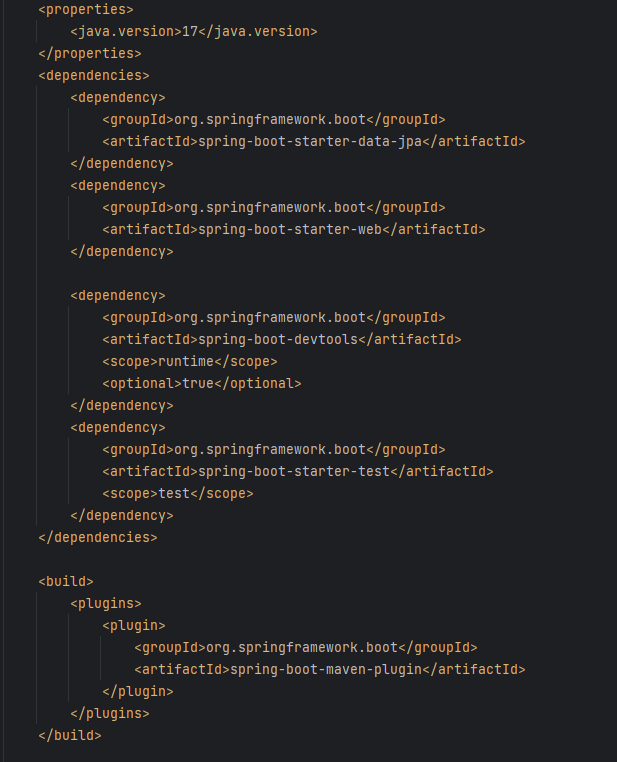
\includegraphics[width=0.70\columnwidth]{foto_pom_base} 
    \caption{Snippet pom.xml generato}
\end{figure}

Rispetto al file utilizzato nel progetto mancano le seguenti dipendenze:
\begin{itemize}
\item \textit{spring-boot-starter-jdbc}, per avviare Spring con il supporto JDBC nel progetto;
\item \textit{mssql-jdbc}, contenente il driver JDBC di Microsoft SQL Server;
\item \hypertarget{doc-api}{\textit{springdoc-openapi-starter-webmvc-ui}}, dipendenza per l'integrazione di Springdoc OpenAPI con Spring Boot per generare la documentazione dell'API utilizzando l'interfaccia utente WebMvc UI;
\item \textit{poi} e \textit{poi-ooxml}, due dipendenze relative ad Apache POI che offre funzionalità per poter lavorare con documenti Microsoft Office;
\item \textit{jxls-jexcel}, dipendenza che include la libreria jXLS per creare e manipolare documenti Excel;
\item \textit{fastexcel} e \textit{fastexcel-reader}, altre dipendenze inerenti a file Excel che offrono funzionalità per lettura,scrittura e modifica di questi file.
\end{itemize}
Per il testing sono state aggiunte:
\begin{itemize}
\item \textit{junit}, framework usato in Java per scrivere test unitari;
\item \textit{hamcrest-library}, libreria utile a scrivere asserzioni più espressive e comprensibili nei test unitari;
\item \textit{h2}, si tratta della dipendenza per la libreria H2 Database Engine, che è un database SQL. Utilizzato con scope "test" per crearne un'istanza temporanea e utilizzarlo nei test.
\end{itemize}

\subsubsection{Application.properties}
\noindent Il secondo file qui sotto rappresentato è il file configurazione \textit{application.properties}. Di seguito riporto il file che ho utilizzato nel progetto:
\begin{figure}[H] 
    \centering 
    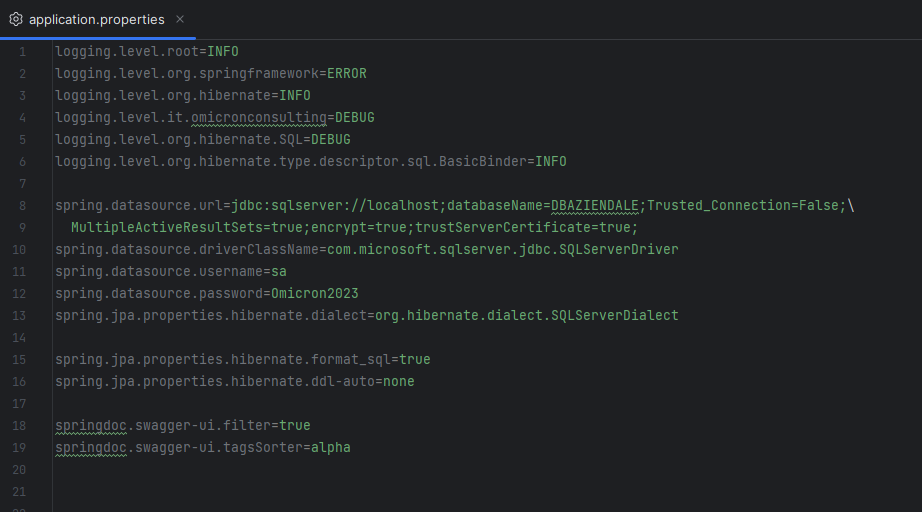
\includegraphics[width=0.85\columnwidth]{foto_application_properties} 
    \caption{Foto application.properties configurato e utilizzato}
\end{figure}

\noindent Possiamo notare come il file utilizzi un formato di configurazione basato su chiavi e valori. Le chiavi rappresentano le diverse proprietà di configurazione dell'applicazione, mentre i valori rappresentano le impostazioni specifiche.\\
Nel file possiamo notare le seguenti chaivi:
\begin{itemize}
\item \textit{logging.level}, servono per configurare il livello di dettaglio dei log per diverse classi o package all'interno dell'applicazione;
\item \textit{spring.datasource}, servono per collegarsi ad un database, in questo caso locale, inserendo username e password e driver di MSSQL;
\item \textit{spring.jpa.properties.hibernate}, serveono per configurare le impostazioni di Hibernate tra cui la validazione schema-entità, il dialetto\textsubscript{g} del server SQL e il suo livello di log;
\item \textit{springdoc.swagger-ui}, libreria che fornisce integrazione tra Spring Boot e Swagger UI.  
\end{itemize}. 








